\documentclass{standalone}
% 

% \pgfmathdeclarefunction{gauss}{2}{%
%   \pgfmathparse{1/(#2*sqrt(2*pi))*exp(-((x-#1)^2)/(2*#2^2))}%
% }
\usepackage{tkz-euclide}
\usetkzobj{all}
\renewcommand{\familydefault}{\sfdefault}
\usepackage{calc,tikz}
\usetikzlibrary{calc}
\usepackage{pgfplots}
\begin{document}
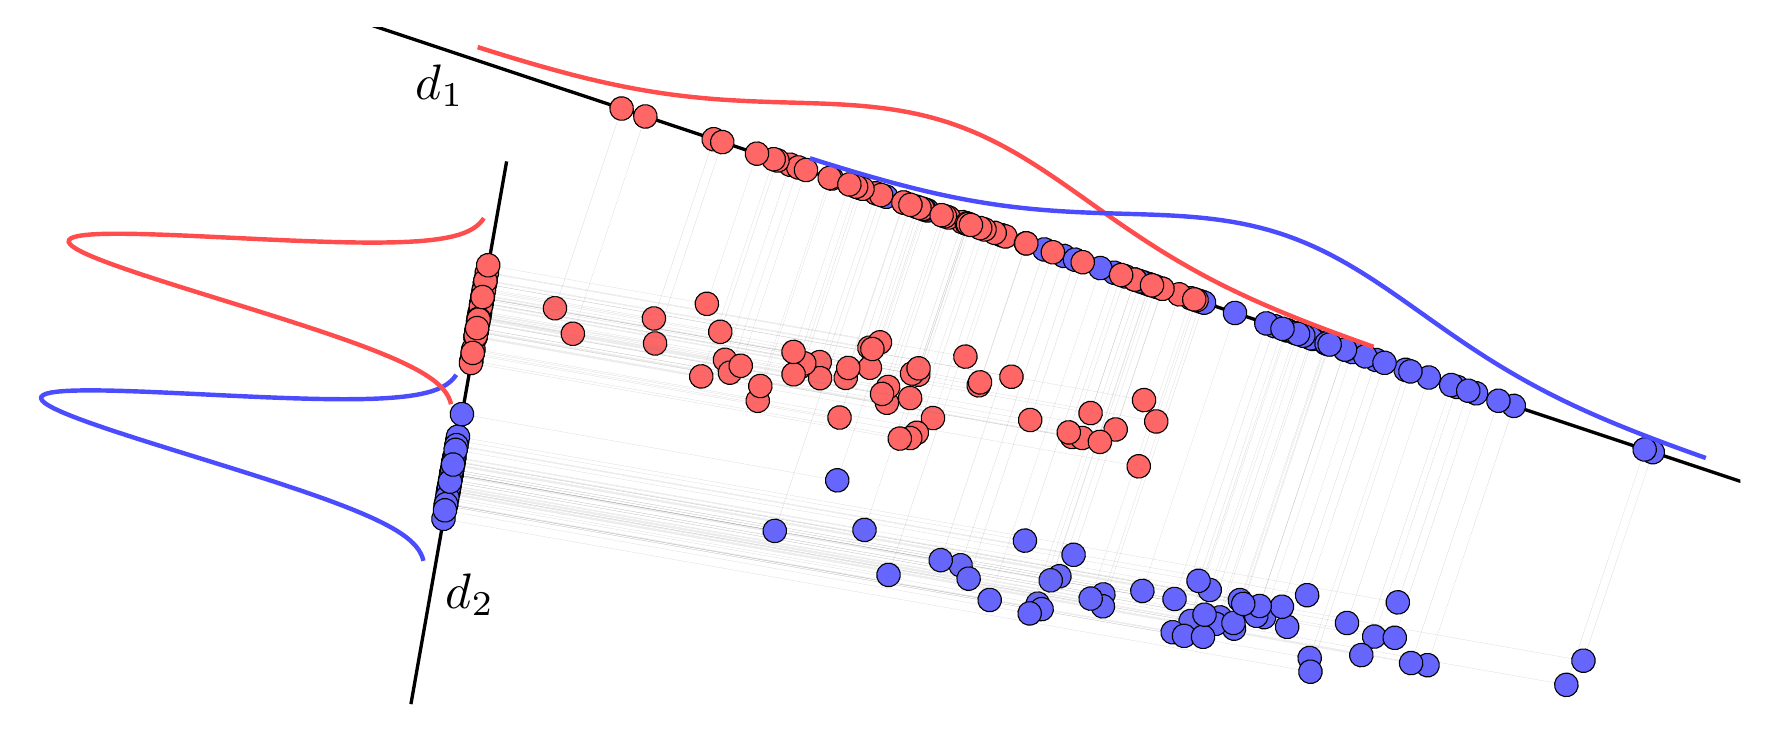
\begin{tikzpicture}[>=stealth]
    \clip (-14.25, -1.4) rectangle (7.5, 7.2);
    \def\normaltwo{\x,{4*1/exp(((\x-0)^2)/2)}}
    % \node [scale = 2] at (6.5, 3.3) {PCA procedure};
    %%%%%%%%% block 1%%%%%%%%%%%%%%%%%
    \begin{scope}[rotate = -10]
    \tkzDefPoint(-15, 6){A}
    \tkzDefPoint(12, 2){B}
    \tkzDefPoint(-9, 4){C}
    \tkzDefPoint(-9, -3){D}
    \draw [ very thick] (A) -- (B);
    \draw [ very thick] (C) -- (D);


    \begin{scope}
        % \draw [rounded corners = 2pt, thick] (-2.7, -3.2) rectangle (3.3, 2.75);
        \begin{scope}[rotate = 0]
            \foreach \x/\y/\z in {0.57/-0.24/0, 2.14/-0.44/1, 2.9/-0.03/2, -1.38/-0.36/3, 1.14/0.13/4, 1.48/-0.03/5, -1.17/0.03/6, -2.43/-0.05/7, -1.68/0.4/8, 0.93/-0.13/9, -1.04/0.33/10, -1.27/-0.04/11, 1.13/-0.24/12, 2.53/0.08/13, 3.16/0.0/14, 5.57/0.13/15, 0.37/-0.42/16, 0.52/-0.44/17, -0.58/-0.1/18, 1.79/-0.1/19, -0.56/-0.25/20, -0.73/-0.18/21, 3.63/-0.27/22, -2.3/-0.2/23, 2.18/-0.61/24, 2.78/-0.29/25, -1.99/-0.42/26, 0.89/-0.22/27, 0.32/0.0/28, -4.83/-0.03/29, 0.76/-0.41/30, -2.69/-0.03/31, 3.12/0.45/32, 3.42/-0.28/33, 1.11/-0.17/34, 1.38/-0.03/35, -3.71/0.18/36, -4.16/0.74/37, 5.41/-0.21/38, -0.1/0.03/39, 0.74/0.19/40, -3.31/-0.33/41, 1.68/0.14/42, -1.32/-0.42/43, 0.73/-0.13/44, 1.97/0.34/45, 1.4/0.1/46, 0.58/0.28/47, -1.46/-0.5/48, 1.19/0.09/49
             } {
                % \draw [fill = blue] (\x, \y) circle (1mm); 
                \tkzDefPoint(\x, \y){x\z}
                \tkzDefPointBy[projection=onto B--A](x\z)
                \tkzGetPoint{H\z}
                \tkzDrawLines[add = 0 and 0, ultra thin, gray, opacity = .3](x\z,H\z)
                \draw [ultra thin, gray, opacity = .3] (-9, \y) -- (\x, \y);
                \draw [fill = blue!60] (\x, \y) circle (1.5mm); 
                \draw [fill = blue!60] (H\z) circle (1.5mm); 

                \draw [fill = blue!60] (-9, \y) circle (1.5mm); 
                % \draw [fill = red] (\x-2, \y+2) circle (1mm); 

                }
        \end{scope}

        \begin{scope}[rotate = 0, xshift  = -4cm, yshift = 2cm]
            \foreach \x/\y/\z in {-0.28/0.04/0, 0.62/0.24/1, 1.17/0.57/2, -0.05/0.47/3, -0.64/0.18/4, 0.54/0.24/5, 0.07/0.56/6, -4.07/0.27/7, 1.4/0.24/8, 3.5/0.42/9, -2.81/0.36/10, -0.88/0.07/11, 0.9/-0.27/12, -2.74/0.05/13, 0.29/-0.18/14, -1.83/0.0/15, -0.6/-0.02/16, 3.7/0.18/17, 2.68/-0.2/18, 3.21/-0.01/19, 0.27/0.02/20, 0.73/-0.49/21, 0.0/0.22/22, 2.86/0.14/23, -1.33/-0.44/24, 0.66/-0.57/25, -0.27/0.17/26, 0.21/-0.08/27, -3.79/-0.01/28, 2.12/-0.08/29, -0.83/0.13/30, 1.41/0.28/31, -1.74/-0.15/32, 0.61/0.32/33, 2.81/-0.19/34, 1.79/0.42/35, 0.57/-0.07/36, -1.95/0.34/37, -0.01/0.46/38, 3.58/-0.42/39, -0.94/-0.03/40, -2.09/-0.26/41, 3.04/-0.2/42, 0.53/-0.6/43, -1.33/-0.25/44, -1.62/-0.04/45, -0.27/-0.47/46, -0.99/0.25/47, -2.18/0.66/48, 2.63/-0.15/49
            } {
                \tkzDefPoint(\x, \y){x\z}
                \tkzDefPointBy[projection=onto B--A](x\z)
                \tkzGetPoint{K\z}
                \draw [ultra thin, gray, opacity = .3] (-5, \y) -- (\x, \y);
                \tkzDrawLines[add = 0 and 0, ultra thin, gray, opacity = .3](x\z,K\z)
                \draw [fill = red!60] (\x, \y) circle (1.5mm); 
                \draw [fill = red!60] (-5, \y) circle (1.5mm); 
                \draw [fill = red!60] (K\z) circle (1.5mm); 

                }
        \end{scope}

        \begin{scope}[yscale = .4, xscale = -1.3, rotate = 270, yshift = 7cm, xshift = -.05cm]
            \draw[color=blue!70,,domain=-3:3, samples = 100, ultra thick] plot (\normaltwo) node[right] {};
            
        \end{scope}

        \begin{scope}[yscale = .4, xscale = -1.3, rotate = 270, yshift = 7cm, xshift = -5.1cm]
            \draw[color=red!70,,domain=-3:3, samples = 100, ultra thick] plot (\normaltwo) node[right] {};
            
        \end{scope}

        \begin{scope}[rotate = -8.5]
            \begin{scope}[yscale = .25, yshift = 15.5cm, xshift = -4.3cm, xscale = 2]
                \draw[color=red!70,,domain=-3:3, samples = 100, ultra thick] plot (\normaltwo) node[right] {};
            \end{scope}
            \begin{scope}[yscale = .25, yshift = 15.5cm, xshift = 0.15cm, xscale = 2]
                \draw[color=blue!70,,domain=-3:3, samples = 100, ultra thick] plot (\normaltwo) node[right] {};
            \end{scope}
        \end{scope}
    \end{scope}

   \node [scale = 1.8] at  (-8.5, -1.5) {$d_2$};
   \node [scale = 1.8] at  (-10, 4.8) {$d_1$};
   \end{scope}

    

\end{tikzpicture}
\end{document}